Esta parte del trabajo practico, tiene como objetivo graficar y determinar la respuesta en frecuencia del amplificador, además de medir su ancho de banda. Los puntos de mayor interés serán las curvas de subida y bajada de ganancia que, generalmente, son marcadas por un cambio de tendencia cuando la respuesta del amplificador es de $-3\mathrm{dB}$ en comparación de su ganancia máxima en máxima excursión simétrica. Las frecuencias que generan una respuesta de $-3\mathrm{dB}$ se nombran como frecuencias de corte. La diferencia entre las frecuencias de corte da como resultado el ancho de banda del amplificador.

Teniendo en cuenta esto se ajusto la señal de entrada al amplificador, tanto a lazo abierto como a lazo cerrado, para obtener la señal de salida en máxima excursión simétrica. Luego matemáticamente se obtuvieron los valores de tensión esperados en la salida para las frecuencias de corte.

Se determino que en nivel de tensión ($V_{pp}$) de la señal de salida a lazo abierto sin saturación es de $V_{ppS}=7V$.Esta señal de salida le corresponde a una señal de entrada de $V_{ppE}=170mV$.
Teniendo en cuenta la ecuación para determinar la ganancia en $dB$ de tensión \ref{eq:dBaveces}, se calculo el nivel esperado de tensión ($V_{out}$) para las frecuencias de corte a lazo abierto:
\begin{equation}
    V_{out}=7V\cdot10^{\frac{-3}{20}}\lrah V_{out}=4,95V
\end{equation}

Se realizo el barrido de frecuencia y se determinaron las frecuencias de corte.
\begin{table}[H]
\parbox{.45\textwidth}{  
    \centering
    \begin{tabular}{|c|c|c|}
        \hline
        $f$ [Hz] &  $V_{pp}$&$GR_{dB}$\\
        \hline
         $750$&$6,92$&$-0.10$\\ 
         $500$&$6,76$&$-0.30$\\ 
         $250$&$6,52$&$-0.62$\\ 
         $150$&$6,28$&$-0.94$\\ 
         $100$&$6,00$&$-1.34$\\ 
         $75$&$5,56$&$-2.00$\\
         $65$&$5,32$&$-2.38$\\
         $54$&$4,96$&$-2.99$\\
         \hline
    \end{tabular}
    \caption{Barrido descendente}
    \label{tab:RF-LAAinf}
    }
    \parbox{.45\textwidth}{
    \centering
    \begin{tabular}{|c|c|c|}
        \hline
        $f$ [kHz] &  $V_{pp}$&$GR_{dB}$\\
        \hline
         $10$&$7,00$&$-0.00$\\ 
         $30$&$6,90$&$-0.12$\\ 
         $50$&$6,28$&$-0.94$\\ 
         $60$&$5,88$&$-1.51$\\ 
         $70$&$5,56$&$-2.00$\\
         $75$&$5,36$&$-2.32$\\
         $78$&$5,28$&$-2.45$\\
         $80$&$5,24$&$-2.51$\\
         $85$&$5,00$&$-2.92$\\
         $87$&$4,96$&$-2.99$\\
         \hline
    \end{tabular}
    \caption{Barrido ascendente}
    \label{tab:RF-LAAsup}
    }
\end{table}
Como se observa en las tablas \ref{tab:RF-LAAinf} y \ref{tab:RF-LAAsup}, la frecuencia de corte correspondiente a la curva de subida de ganancia es de $F_{CAinf}=54_{Hz}$ y la frecuencia de corte correspondiente a la curva de bajada de ganancia es de $F_{CAsup}=87_{kHz}$. Dando como resultado un ancho de banda de:
\begin{equation*}
    AB_{LA} = F_{CAsup}-F_{CAinf}\lrah AB_{LA}=86.946 kHz
\end{equation*}

\begin{figure}[H]
    \centering
    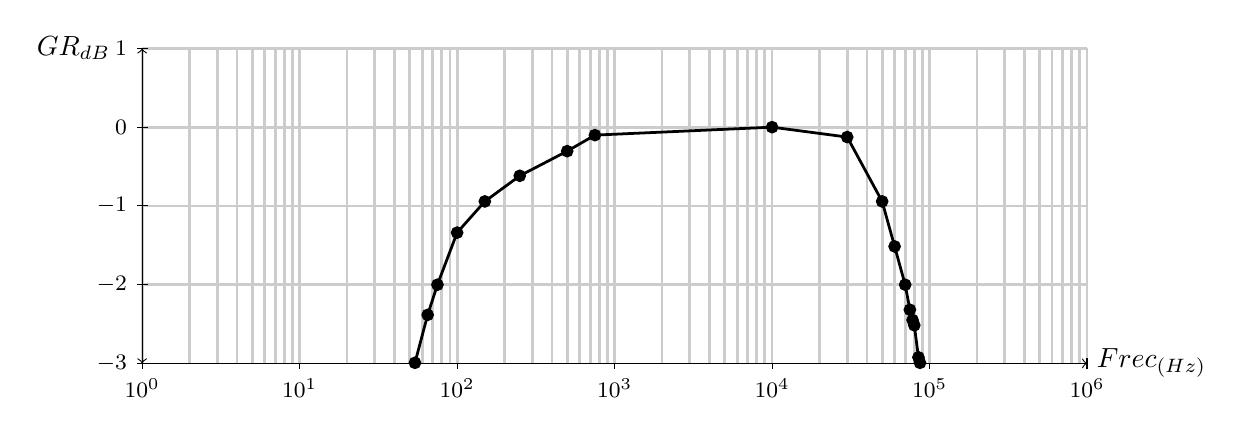
\begin{tikzpicture}[scale=1]

    \def\scalya{3}
    \def\scaly{1}
    \def\scalxa{3}
    \def\scalx{2}
    
    %datosLineaA
    \coordinate (a8) at ({log10(750)*\scalx},{20*log10(6.92/7)*\scaly+\scalya});
    \coordinate (a7) at ({log10(500)*\scalx},{20*log10(6.76/7)*\scaly+\scalya});
    \coordinate (a6) at ({log10(250)*\scalx},{20*log10(6.52/7)*\scaly+\scalya});
    \coordinate (a5) at ({log10(150)*\scalx},{20*log10(6.28/7)*\scaly+\scalya});
    \coordinate (a4) at ({log10(100)*\scalx},{20*log10(6.00/7)*\scaly+\scalya});
    \coordinate (a3) at ({log10(75)*\scalx},{20*log10(5.56/7)*\scaly+\scalya});
    \coordinate (a2) at ({log10(65)*\scalx},{20*log10(5.32/7)*\scaly+\scalya});
    \coordinate (a1) at ({log10(54)*\scalx},{20*log10(4.96/7)*\scaly+\scalya});
    \coordinate (a9) at ({(log10(10)+\scalxa)*\scalx},{20*log10(7.00/7)*\scaly+\scalya});
    \coordinate (a10) at ({(log10(30)+\scalxa)*\scalx},{20*log10(6.90/7)*\scaly+\scalya});
    \coordinate (a11) at ({(log10(50)+\scalxa)*\scalx},{20*log10(6.28/7)*\scaly+\scalya});
    \coordinate (a12) at ({(log10(60)+\scalxa)*\scalx},{20*log10(5.88/7)*\scaly+\scalya});
    \coordinate (a13) at ({(log10(70)+\scalxa)*\scalx},{20*log10(5.56/7)*\scaly+\scalya});
    \coordinate (a14) at ({(log10(75)+\scalxa)*\scalx},{20*log10(5.36/7)*\scaly+\scalya});
    \coordinate (a15) at ({(log10(78)+\scalxa)*\scalx},{20*log10(5.28/7)*\scaly+\scalya});
    \coordinate (a16) at ({(log10(80)+\scalxa)*\scalx},{20*log10(5.24/7)*\scaly+\scalya});
    \coordinate (a17) at ({(log10(85)+\scalxa)*\scalx},{20*log10(5.00/7)*\scaly+\scalya});
    \coordinate (a18) at ({(log10(87)+\scalxa)*\scalx},{20*log10(4.96/7)*\scaly+\scalya});



    
    %Ejex
    \foreach \x [evaluate={\a=int(\x+1)}]in {0,...,5}{
    \foreach \y in {1,...,10}
        \draw[line width=1pt,gray!40] ({(\x+log10(\y))*\scalx},0)--({(\x+log10(\y))*\scalx},4);
        \draw[shift={(\a*\scalx,0)}] (0pt,2pt) -- (0pt,-2pt) node[below] {\footnotesize $10^\a$};
    }
    \draw[shift={(0,0)}] (0pt,2pt) -- (0pt,-2pt) node[below] {\footnotesize $10^0$};
    \draw[->] (0,0)--(12,0) node[right] {$Frec_{(Hz)}$};
    
    %Ejey
    \foreach \y [evaluate={\a=int(\y-3)}] in {1,...,4}{
        \draw[line width=1pt,gray!40] (0,\y)--(12,\y);
        \draw[shift={(0,\y)}] (2pt,0pt) -- (-2pt,0pt) node [left] {\footnotesize $\a$};
    }
   \draw[shift={(0,0)}] (2pt,0pt) -- (-2pt,0pt) node [left] {\footnotesize $-3$};
   \draw[<->] (0,0)--(0,4) node[left=8pt]{$GR_{dB}$};
   
   
    %Linea A
    \foreach \x  in {1,...,18}{
        \draw[line width=1.5pt,fill=black] (a\x) circle(1.5pt);
   }
   \foreach \x [evaluate={\y=int(\x+1);}] in {1,...,17}{
        \draw[line width=1pt,black] (a\x) -- (a\y);
   }
   
\end{tikzpicture}
    \caption{Respuesta en frecuencia de ganancia relativa a lazo abierto}
    \label{fig:RFA}
\end{figure}
Se repitió el mismo procedimiento para el caso de la configuración a lazo cerrado. Se observo que el valor máximo de tensión pico-pico a la salida en la configuración de lazo cerrado, que no genere distorsión, es de  $V_{ppS}=7.48$, correspondiente a una señal de tensión pico-pico a la entrada de $V_{ppE}=3.2$. Utilizando la ecuación \ref{eq:dBaveces} se obtuvo el nivel de tensión esperado a la salida para las frecuencias de corte:
\begin{equation}
    V_{out}=7.48V\cdot10^{\frac{-3}{20}}\lrah V_{out}=5,29V
\end{equation}
Se realizo el barrido de frecuencia obteniendo las siguientes tablas de datos.
\begin{table}[H]
\parbox{.45\textwidth}{  
    \centering
   \begin{tabular}{|c|c|c|}
        \hline
        $f$ [Hz] &  $V_{pp}$ & $GR_{dB}$\\
        \hline
         $500$&$7,48$&$0$\\ 
         $250$&$7,40$&$-0.09$\\ 
         $150$&$7,40$&$-0.09$\\ 
         $100$&$7,32$&$-0.19$\\ 
         $50$&$7,08$&$-0.48$\\
         $30$&$6,92$&$-0.67$\\
         $25$&$6,76$&$-0.88$\\
         $20$&$6,52$&$-1.19$\\
         $15$&$6,12$&$-1.74$\\
         $13$&$5,96$&$-1.97$\\
         $11$&$5,46$&$-2.73$\\
         $10$&$5,28$&$-3.02$\\
         \hline
    \end{tabular}
    \caption{Barrido descendente}
    \label{tab:RF-LACinf}
    }
    \parbox{.45\textwidth}{
    \centering
    \begin{tabular}{|c|c|c|}
        \hline
        $f$ [kHz] &  $V_{pp}$&$GR_{dB}$\\
        \hline
         $30$&$7,48$&$0$\\ 
         $50$&$7,50$&$0.05$\\ 
         $100$&$7,46$&$0.05$\\ 
         $150$&$7,44$&$0.05$\\
         $250$&$7,40$&$-0.09$\\
         $350$&$7,36$&$-0.14$\\
         $400$&$7,32$&$-0.19$\\
         $500$&$7,24$&$-0.28$\\
         $700$&$7,00$&$-0.58$\\
         $1000$&$6,47$&$-1.26$\\
         $1500$&$5,66$&$-2.42$\\
         $1770$&$5,28$&$-3.02$\\
         \hline
    \end{tabular}
    \caption{Barrido ascendente}
    \label{tab:RF-LACsup}
    }
\end{table}
De las tablas \ref{tab:RF-LACinf} y \ref{tab:RF-LACsup} se obtuvieron ambas frecuencias de corte. La frecuencia de corte inferior es de $F_{CCinf}=10_{Hz}$ y la frecuencia de corte superior es de $F_{CCsup}=1.773_{MHz}$. Esto da como resultado un ancho de banda de:
\begin{equation*}
    AB_{LC} = F_{CCsup}-F_{CCinf}\lrah AB_{LA}=1.77299 MHz
\end{equation*}
\begin{figure}[H]
    \centering
    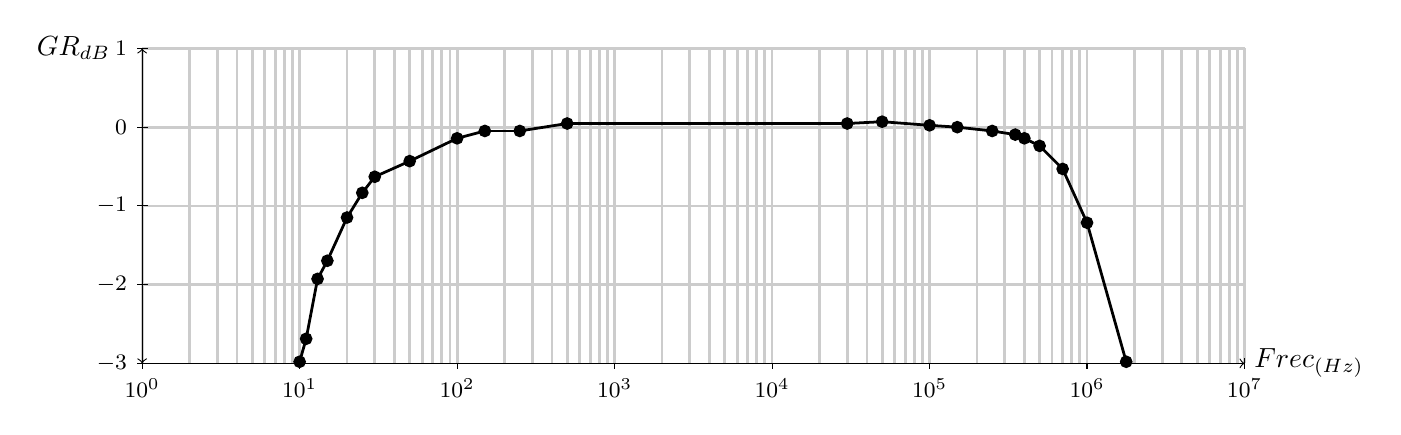
\begin{tikzpicture}[scale=1]

    \def\scalya{3}
    \def\scaly{1}
    \def\scalx{2}
    \def\scalxa{3}
    
    %datosLineaA
    \coordinate (a1) at ({\scalx*log10(10)}, {\scaly*(20*log10(5.28/7.44) + \scalya)});
    \coordinate (a2) at ({\scalx*log10(11)}, {\scaly*(20*log10(5.46/7.44) + \scalya)});
    \coordinate (a3) at ({\scalx*log10(13)}, {\scaly*(20*log10(5.96/7.44) + \scalya)});
    \coordinate (a4) at ({\scalx*log10(15)}, {\scaly*(20*log10(6.12/7.44) + \scalya)});
    \coordinate (a5) at ({\scalx*log10(20)}, {\scaly*(20*log10(6.52/7.44) + \scalya)});
    \coordinate (a6) at ({\scalx*log10(25)}, {\scaly*(20*log10(6.76/7.44) + \scalya)});
    \coordinate (a7) at ({\scalx*log10(30)}, {\scaly*(20*log10(6.92/7.44) + \scalya)});
    \coordinate (a8) at ({\scalx*log10(50)}, {\scaly*(20*log10(7.08/7.44) + \scalya)});
    \coordinate (a9) at ({\scalx*log10(100)}, {\scaly*(20*log10(7.32/7.44) + \scalya)});
    \coordinate (a10) at ({\scalx*log10(150)}, {\scaly*(20*log10(7.40/7.44) + \scalya)});
    \coordinate (a11) at ({\scalx*log10(250)}, {\scaly*(20*log10(7.40/7.44) + \scalya)});
    \coordinate (a12) at ({\scalx*log10(500)}, {\scaly*(20*log10(7.48/7.44) + \scalya)});
    \coordinate (a13) at ({\scalx*(log10(30) + \scalxa)}, {\scaly*(20*log10(7.48/7.44) + \scalya)});
    \coordinate (a14) at ({\scalx*(log10(50) + \scalxa)}, {\scaly*(20*log10(7.50/7.44) + \scalya)});
    \coordinate (a15) at ({\scalx*(log10(100) + \scalxa)}, {\scaly*(20*log10(7.46/7.44) + \scalya)});
    \coordinate (a16) at ({\scalx*(log10(150) + \scalxa)}, {\scaly*(20*log10(7.44/7.44) + \scalya)});
    \coordinate (a17) at ({\scalx*(log10(250) + \scalxa)}, {\scaly*(20*log10(7.40/7.44) + \scalya)});
    \coordinate (a18) at ({\scalx*(log10(350) + \scalxa)}, {\scaly*(20*log10(7.36/7.44) + \scalya)});
    \coordinate (a19) at ({\scalx*(log10(400) + \scalxa)}, {\scaly*(20*log10(7.32/7.44) + \scalya)});
    \coordinate (a20) at ({\scalx*(log10(500) + \scalxa)}, {\scaly*(20*log10(7.24/7.44) + \scalya)});
    \coordinate (a21) at ({\scalx*(log10(700) + \scalxa)}, {\scaly*(20*log10(7.00/7.44) + \scalya)});
    \coordinate (a22) at ({\scalx*(log10(1000) + \scalxa)}, {\scaly*(20*log10(6.47/7.44) + \scalya)});
    \coordinate (a23) at ({\scalx*(log10(1500) + \scalxa)}, {\scaly*(20*log10(5.66/7.44) + \scalya)});
    \coordinate (a23) at ({\scalx*(log10(1773) + \scalxa)}, {\scaly*(20*log10(5.28/7.44) + \scalya)});

    
    %Ejex
    \foreach \x [evaluate={\a=int(\x+1)}]in {0,...,6}{
    \foreach \y in {1,...,10}
        \draw[line width=1pt,gray!40] ({(\x+log10(\y))*\scalx},0)--({(\x+log10(\y))*\scalx},4);
        \draw[shift={(\a*\scalx,0)}] (0pt,2pt) -- (0pt,-2pt) node[below] {\footnotesize $10^\a$};
    }
    \draw[shift={(0,0)}] (0pt,2pt) -- (0pt,-2pt) node[below] {\footnotesize $10^0$};
    \draw[->] (0,0)--(14,0) node[right] {$Frec_{(Hz)}$};
    
    %Ejey
    \foreach \y [evaluate={\a=int(\y-3)}] in {1,...,4}{
        \draw[line width=1pt,gray!40] (0,\y*\scaly)--(14,\y*\scaly);
        \draw[shift={(0,\y*\scaly)}] (2pt,0pt) -- (-2pt,0pt) node [left] {\footnotesize $\a$};
    }
   \draw[shift={(0,0)}] (2pt,0pt) -- (-2pt,0pt) node [left] {\footnotesize $-3$};
   \draw[<->] (0,0)--(0,4) node[left=8pt]{$GR_{dB}$};
   
   
    %Linea A
    \foreach \x  in {1,...,23}{
        \draw[line width=1.5pt,fill=black] (a\x) circle(1.5pt);
   }
   \foreach \x [evaluate={\y=int(\x+1);}] in {1,...,22}{
        \draw[line width=1pt,black] (a\x) -- (a\y);
   }
   
\end{tikzpicture}
    \caption{Respuesta en frecuencia de ganancia relativa a lazo cerrado}
    \label{fig:RFC}
\end{figure}

Como es de esperar, el amplificador en la configuración de lazo abierto pose un menor ancho de banda que a lazo cerrado, pero la ganancia se reduce en comparación. Sabiendo cuales eran los niveles de tensión de la señales de entrada para ambas configuraciones, podemos comparar amabas curvas y comprobar su ancho de banda y ganancia.
\begin{figure}[H]
    \centering
    \begin{tikzpicture}[scale=1]

    \def\scalya{0}%Desfase curvas
    \def\scaly{1/5}%Escala eje y
    \def\scalx{2}%Escala eje x
    \def\scalxa{3}%Desfase puntos kHz
    
    %datosLineaA
    \coordinate (a1) at ({\scalx*log10(10)}, {\scaly*(20*log10(5.28/3.2) + \scalya)});
    \coordinate (a2) at ({\scalx*log10(11)}, {\scaly*(20*log10(5.46/3.2) + \scalya)});
    \coordinate (a3) at ({\scalx*log10(13)}, {\scaly*(20*log10(5.96/3.2) + \scalya)});
    \coordinate (a4) at ({\scalx*log10(15)}, {\scaly*(20*log10(6.12/3.2) + \scalya)});
    \coordinate (a5) at ({\scalx*log10(20)}, {\scaly*(20*log10(6.52/3.2) + \scalya)});
    \coordinate (a6) at ({\scalx*log10(25)}, {\scaly*(20*log10(6.76/3.2) + \scalya)});
    \coordinate (a7) at ({\scalx*log10(30)}, {\scaly*(20*log10(6.92/3.2) + \scalya)});
    \coordinate (a8) at ({\scalx*log10(50)}, {\scaly*(20*log10(7.08/3.2) + \scalya)});
    \coordinate (a9) at ({\scalx*log10(100)}, {\scaly*(20*log10(7.32/3.2) + \scalya)});
    \coordinate (a10) at ({\scalx*log10(150)}, {\scaly*(20*log10(7.40/3.2) + \scalya)});
    \coordinate (a11) at ({\scalx*log10(250)}, {\scaly*(20*log10(7.40/3.2) + \scalya)});
    \coordinate (a12) at ({\scalx*log10(500)}, {\scaly*(20*log10(7.48/3.2) + \scalya)});
    \coordinate (a13) at ({\scalx*(log10(30) + \scalxa)}, {\scaly*(20*log10(7.48/3.2) + \scalya)});
    \coordinate (a14) at ({\scalx*(log10(50) + \scalxa)}, {\scaly*(20*log10(7.52/3.2) + \scalya)});
    \coordinate (a15) at ({\scalx*(log10(100) + \scalxa)}, {\scaly*(20*log10(7.52/3.2) + \scalya)});
    \coordinate (a16) at ({\scalx*(log10(150) + \scalxa)}, {\scaly*(20*log10(7.52/3.2) + \scalya)});
    \coordinate (a17) at ({\scalx*(log10(250) + \scalxa)}, {\scaly*(20*log10(7.40/3.2) + \scalya)});
    \coordinate (a18) at ({\scalx*(log10(350) + \scalxa)}, {\scaly*(20*log10(7.36/3.2) + \scalya)});
    \coordinate (a19) at ({\scalx*(log10(400) + \scalxa)}, {\scaly*(20*log10(7.32/3.2) + \scalya)});
    \coordinate (a20) at ({\scalx*(log10(500) + \scalxa)}, {\scaly*(20*log10(7.24/3.2) + \scalya)});
    \coordinate (a21) at ({\scalx*(log10(700) + \scalxa)}, {\scaly*(20*log10(7.00/3.2) + \scalya)});
    \coordinate (a22) at ({\scalx*(log10(1000) + \scalxa)}, {\scaly*(20*log10(6.68/3.2) + \scalya)});
    \coordinate (a23) at ({\scalx*(log10(1500) + \scalxa)}, {\scaly*(20*log10(5.96/3.2) + \scalya)});
    \coordinate (a23) at ({\scalx*(log10(2000) + \scalxa)}, {\scaly*(20*log10(5.28/3.2) + \scalya)});
    %datosLineaB
    \coordinate (b8) at ({log10(750)*\scalx},{(20*log10(6.92/0.17)+\scalya)*\scaly});
    \coordinate (b7) at ({log10(500)*\scalx},{(20*log10(6.76/0.17)+\scalya)*\scaly});
    \coordinate (b6) at ({log10(250)*\scalx},{(20*log10(6.52/0.17)+\scalya)*\scaly});
    \coordinate (b5) at ({log10(150)*\scalx},{(20*log10(6.28/0.17)+\scalya)*\scaly});
    \coordinate (b4) at ({log10(100)*\scalx},{(20*log10(6.00/0.17)+\scalya)*\scaly});
    \coordinate (b3) at ({log10(75)*\scalx},{(20*log10(5.56/0.17)+\scalya)*\scaly});
    \coordinate (b2) at ({log10(65)*\scalx},{(20*log10(5.32/0.17)+\scalya)*\scaly});
    \coordinate (b1) at ({log10(54)*\scalx},{(20*log10(4.96/0.17)+\scalya)*\scaly});
    \coordinate (b9) at ({(log10(10)+\scalxa)*\scalx},{(20*log10(7.00/0.17)+\scalya)*\scaly});
    \coordinate (b10) at ({(log10(30)+\scalxa)*\scalx},{(20*log10(6.90/0.17)+\scalya)*\scaly});
    \coordinate (b11) at ({(log10(50)+\scalxa)*\scalx},{(20*log10(6.28/0.17)+\scalya)*\scaly});
    \coordinate (b12) at ({(log10(60)+\scalxa)*\scalx},{(20*log10(5.88/0.17)+\scalya)*\scaly});
    \coordinate (b13) at ({(log10(70)+\scalxa)*\scalx},{(20*log10(5.56/0.17)+\scalya)*\scaly});
    \coordinate (b14) at ({(log10(75)+\scalxa)*\scalx},{(20*log10(5.36/0.17)+\scalya)*\scaly});
    \coordinate (b15) at ({(log10(78)+\scalxa)*\scalx},{(20*log10(5.28/0.17)+\scalya)*\scaly});
    \coordinate (b16) at ({(log10(80)+\scalxa)*\scalx},{(20*log10(5.24/0.17)+\scalya)*\scaly});
    \coordinate (b17) at ({(log10(85)+\scalxa)*\scalx},{(20*log10(5.00/0.17)+\scalya)*\scaly});
    \coordinate (b18) at ({(log10(87)+\scalxa)*\scalx},{(20*log10(4.96/0.17)+\scalya)*\scaly});
    
    %Ejex
    \foreach \x [evaluate={\a=int(\x+1)}]in {0,...,6}{
    \foreach \y in {1,...,10}
        \draw[line width=1pt,gray!40] ({(\x+log10(\y))*\scalx},0)--({(\x+log10(\y))*\scalx},35*\scaly);
        \draw[shift={(\a*\scalx,0)}] (0pt,2pt) -- (0pt,-2pt) node[below] {\footnotesize $10^\a$};
    }
    \draw[shift={(0,0)}] (0pt,2pt) -- (0pt,-2pt) node[below] {\footnotesize $10^0$};
    \draw[->] (0,0)--(7*\scalx,0) node[right] {$Frec_{(Hz)}$};
    
    %Ejey
    \foreach \y [evaluate={\a=int(\y/(\scaly))}] in {1,...,7}{
        \draw[line width=1pt,gray!40] (0,\y)--(7*\scalx,\y);
        \draw[shift={(0,\y)}] (2pt,0pt) -- (-2pt,0pt) node [left] {\footnotesize $\a$};
    }
   \draw[shift={(0,0)}] (2pt,0pt) -- (-2pt,0pt) node [left] {\footnotesize $0$};
   \draw[<->] (0,0)--(0,35*\scaly) node[left=0.7cm]{$G_{dB}$};
   
   
    %Linea A
    \foreach \x  in {1,...,23}{
        \draw[line width=1.5pt,fill=black] (a\x) circle(1.5pt);
   }
   \foreach \x [evaluate={\y=int(\x+1);}] in {1,...,22}{
        \draw[line width=1pt,black] (a\x) -- (a\y);
   }
   %Linea B
   \foreach \x  in {1,...,18}{
        \draw[line width=1.5pt,fill=mdrd,mdrd] (b\x) circle(1.5pt);
   }
   \foreach \x [evaluate={\y=int(\x+1);}] in {1,...,17}{
        \draw[line width=1pt,mdrd] (b\x) -- (b\y);
   }

   \draw[line width=1pt,mdrd,dashed] (b1)--(1.47*\scalx,0);
   \draw[line width=1pt,mdrd,dashed] (b18)--(5.2*\scalx,0);
   \draw[line width=1pt,black,dashed] (a1)--(0.8*\scalx,0);
   \draw[line width=1pt,black,dashed] (a23)--(6.5*\scalx,0);
   
\end{tikzpicture}
    \caption{Comparación de las respuestas en frecuencia}
    \label{fig:RFcomp}
\end{figure}
Cabe aclarar que las lineas punteadas en el gráfico \ref{fig:RFcomp} son aproximaciones relevadas por la información obtenida en los pasos anteriores y por el comportamiento esperado de un amplificador de este tipo.